% !TEX root = ../../CompVis.tex
\section{Object Detection and Classification}

\subsection{Boosting}
\begin{enumerate}
    \item Input: Trainind data (positive, negative) with weights
    \item For $t=1,\ldots,T$
          \begin{enumerate}
              \item Train a weak classifier
              \item Classify training data
              \item Increase weight on incorrectly classified samples
          \end{enumerate}
    \item Use the weighted combination of all weak classifiers for the final (strong) classifier
\end{enumerate}
Weak classifier: $h_j(x)=\left\{\begin{matrix}1, &p_j f_j < p_j \theta_j\\0 & \text{otherwise}\end{matrix}\right.$, where $f$ features, $\theta$ thresholds, $p$ parity

\subsubsection{Haar Features}
Simple filters of different sizes and shapes with only -1 or 1 in the masks.
Calculate features on sub windows (sliding window).
Find set of important features using AdaBoost (treat them as weak classifiers).

\paragraph{Integral Image}
Fast calculation of filters results by using integral images.
Each pixel in the integral image contains the sum of all pixel values in the indicated rectangle

\begin{minipage}{0.7\textwidth}
    The sum of the pixels within rectangle $D$ can be computed with four array references.
    The value of the integral image at location 1 is the sum of pixels in rectangle $A$.
    The value at location 2 is $A + B$, at location 3 is $A + C$, and at location 4 is $A + B + C + D$.
    The sum within D can be computed as $4 + 1 - (2 + 3)$.
\end{minipage}
\begin{minipage}{0.3\textwidth}
    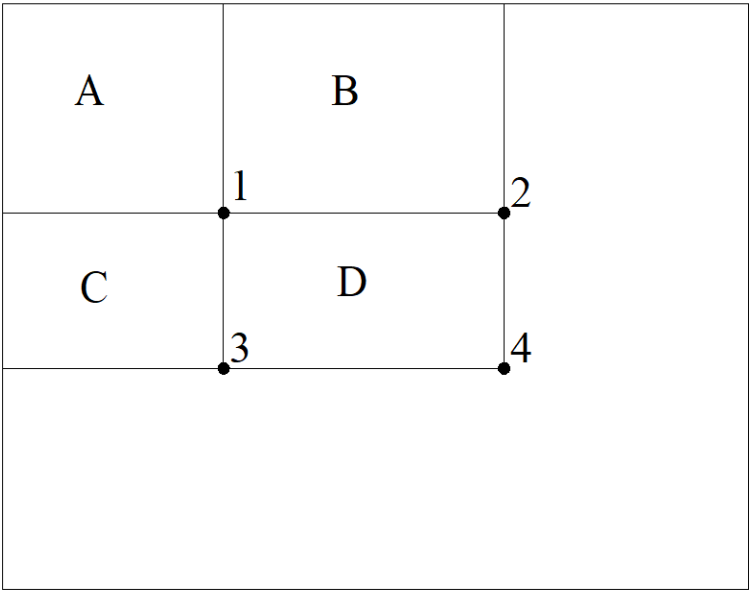
\includegraphics[width=1.0\textwidth]{sections/FindingMultipleObjects/img/integral_image.png}
\end{minipage}

\subsection{Cascaded Classifiers}
\begin{minipage}{0.5\textwidth}
    A sliding window detector needs to evaluate thousand of possible position/scale combinations in the image.
    Using for example $10^6$ pixels should result in a false positive rate of less than $10^{-6}$.
    Idea: Dismiss regions without objects efficiently $\rightarrow$ Cascaded classifiers.

    Example 10 cascades: True positive rate for step: 0.99, false positive rate for step 0.3

    $\Rightarrow$ TPR = $0.99^{10}=0.904$, FPR = $0.3^{10}=0.0000059$
\end{minipage}
\begin{minipage}{0.5\textwidth}
    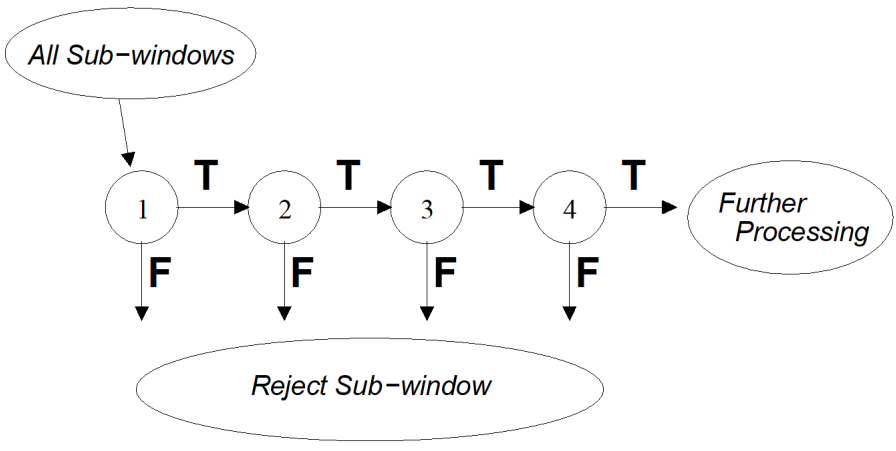
\includegraphics[width=1\textwidth]{sections/FindingMultipleObjects/img/cascaded_classifier.png}
\end{minipage}
\begin{itemize}
    \item Training time for cascade and features take days to weeks (!!)
    \item Fast performance
    \item Long time best face detector
    \item One of the fist widely usable object detection approaches
\end{itemize}

\subsection{Region Proposals}
Find image regions that are likely to contain an object.
Relatively fast for 1000 proposals, some seconds on CPU
\begin{itemize}
    \item Region Segmentation (graph based)
    \item Hierarchical Grouping
\end{itemize}

\subsection{Classic Approaches}
\begin{multicols}{2}
    \subsubsection{Standard Approach}
    \begin{enumerate}
        \item Features
        \item Classifier
        \item Sliding Window
    \end{enumerate}

    \subsubsection{Viola Jones Face-Detector (Faces, Objects)}
    \begin{enumerate}
        \item Haar features
        \item Boosting
        \item Cascaded Classifiers
    \end{enumerate}
\end{multicols}

\subsubsection{Dalal and Triggs HoG Detector (People, Pedestrians)}
\begin{enumerate}
    \item Calculate HoG descriptors (for whole image in blocks)
    \item Collect HoG's in detection window
    \item Use linear SVM for person / non-person Classification
\end{enumerate}
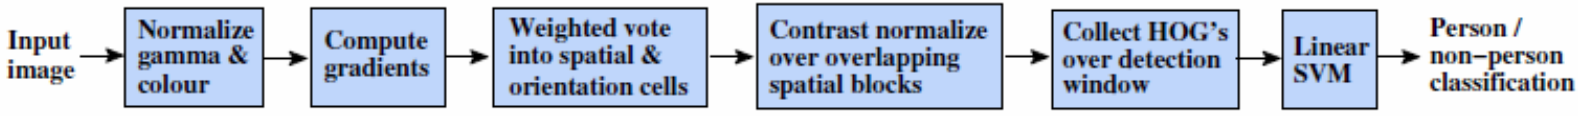
\includegraphics[width=0.9\textwidth]{sections/FindingMultipleObjects/img/dalal_triggs.png}

\subsection{Modern Approaches}
\subsubsection{OverFeat}
Combine classification, localisation and detection
\begin{itemize}
    \item Classification
          \begin{itemize}
              \item CNN (similar to AlexNet)
              \item Sliding window: Apply at every possible pixel and at multiple scales
              \item Subsampling factor of 12 (result every 12th pixel in each axis)
          \end{itemize}
    \item Localisation
          \begin{itemize}
              \item Generate bounding box prediction (as a regression problem)
              \item Uses the same first 5 layers in the CNN
          \end{itemize}
\end{itemize}
\subsubsection{RCNN}
\begin{minipage}{0.5\textwidth}
    \glqq Synergy of deep architectures with classical computer vision\grqq
    \begin{enumerate}
        \item Extract region proposals (are warped to $227\times 227$ images)
        \item Compute CNN features (4096 features from $227\times 227$ images using 5 convolutional and 2 fully connected layers from AlexNet)
        \item Classify regions using SVM (1 per class / 1 vs. all)
    \end{enumerate}
    Supervised pre-training on ILSVRC2012 classfication data set and then domain-specific fine-tuning.
    Regions with overlap of 30\% or more are considered positive examples.

    Incoherent training objectives
    \begin{itemize}
        \item Tune networ with softmax (log loss)
        \item Train linear SVM (hinge loss)
        \item Training bounding box localization (least squares)
    \end{itemize}
    Slow training, slow interference (47s / image with VGG 16 network, faster with SPP-Net)
\end{minipage}
\begin{minipage}{0.5\textwidth}
    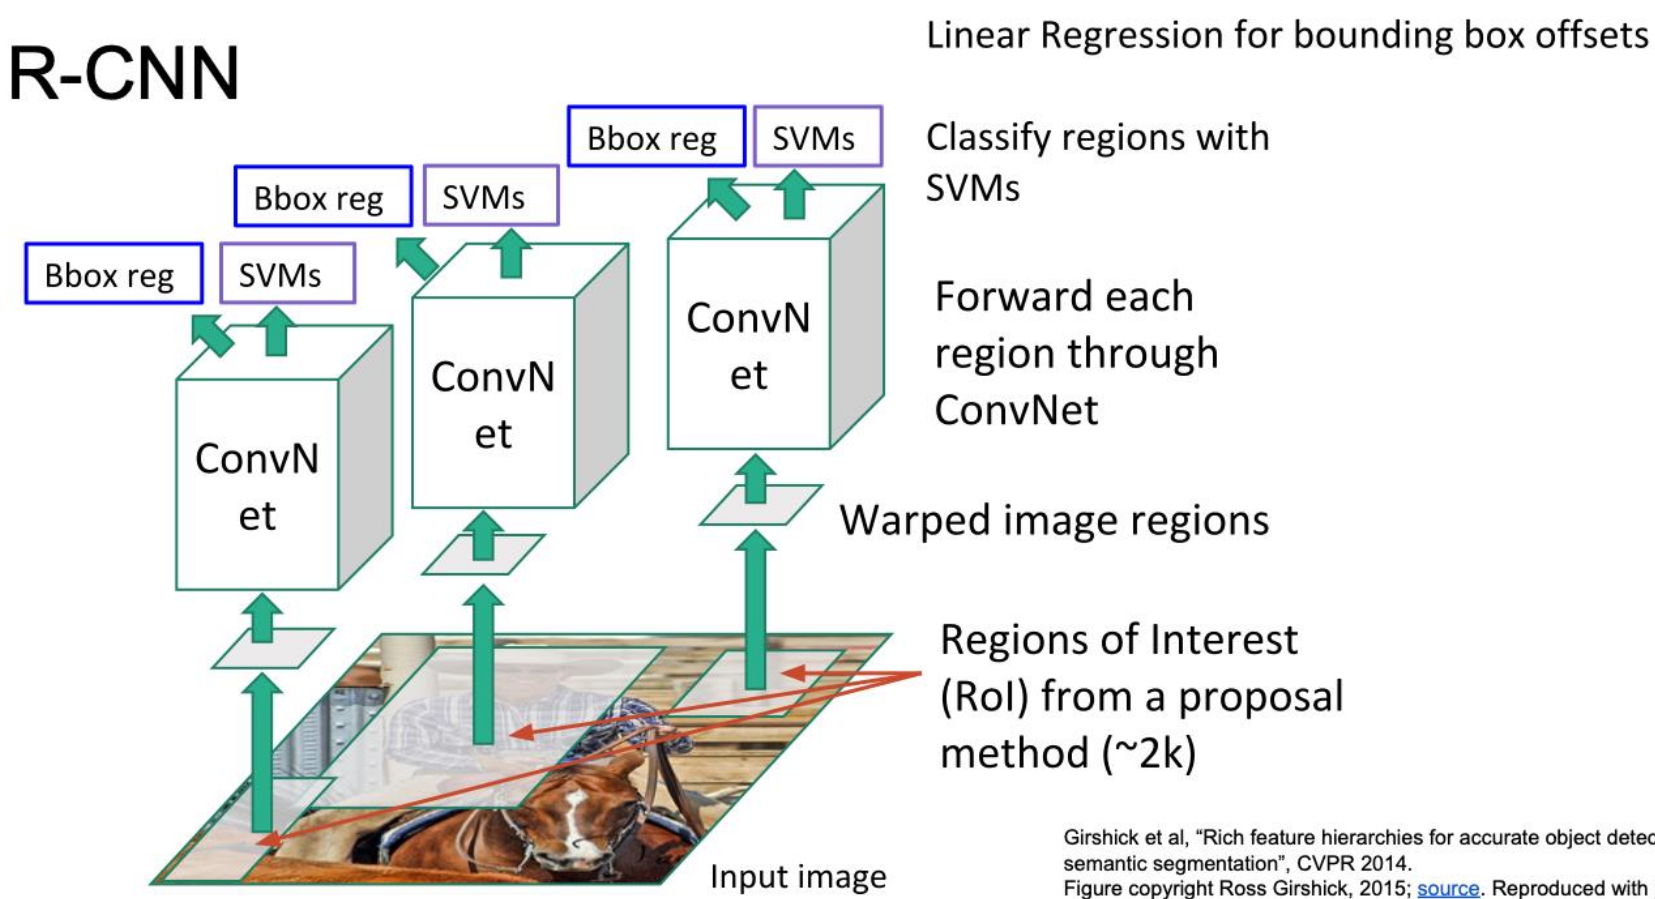
\includegraphics[width=1.0\textwidth]{sections/FindingMultipleObjects/img/rcnn.png}
\end{minipage}
\subsubsection{Fast and Faster RCNN}
\begin{minipage}{0.5\textwidth}
    \paragraph{Fast RCNN}
    Replace SVM of RCNN with fully connected neural network for: Class of object, refined bounding box object

    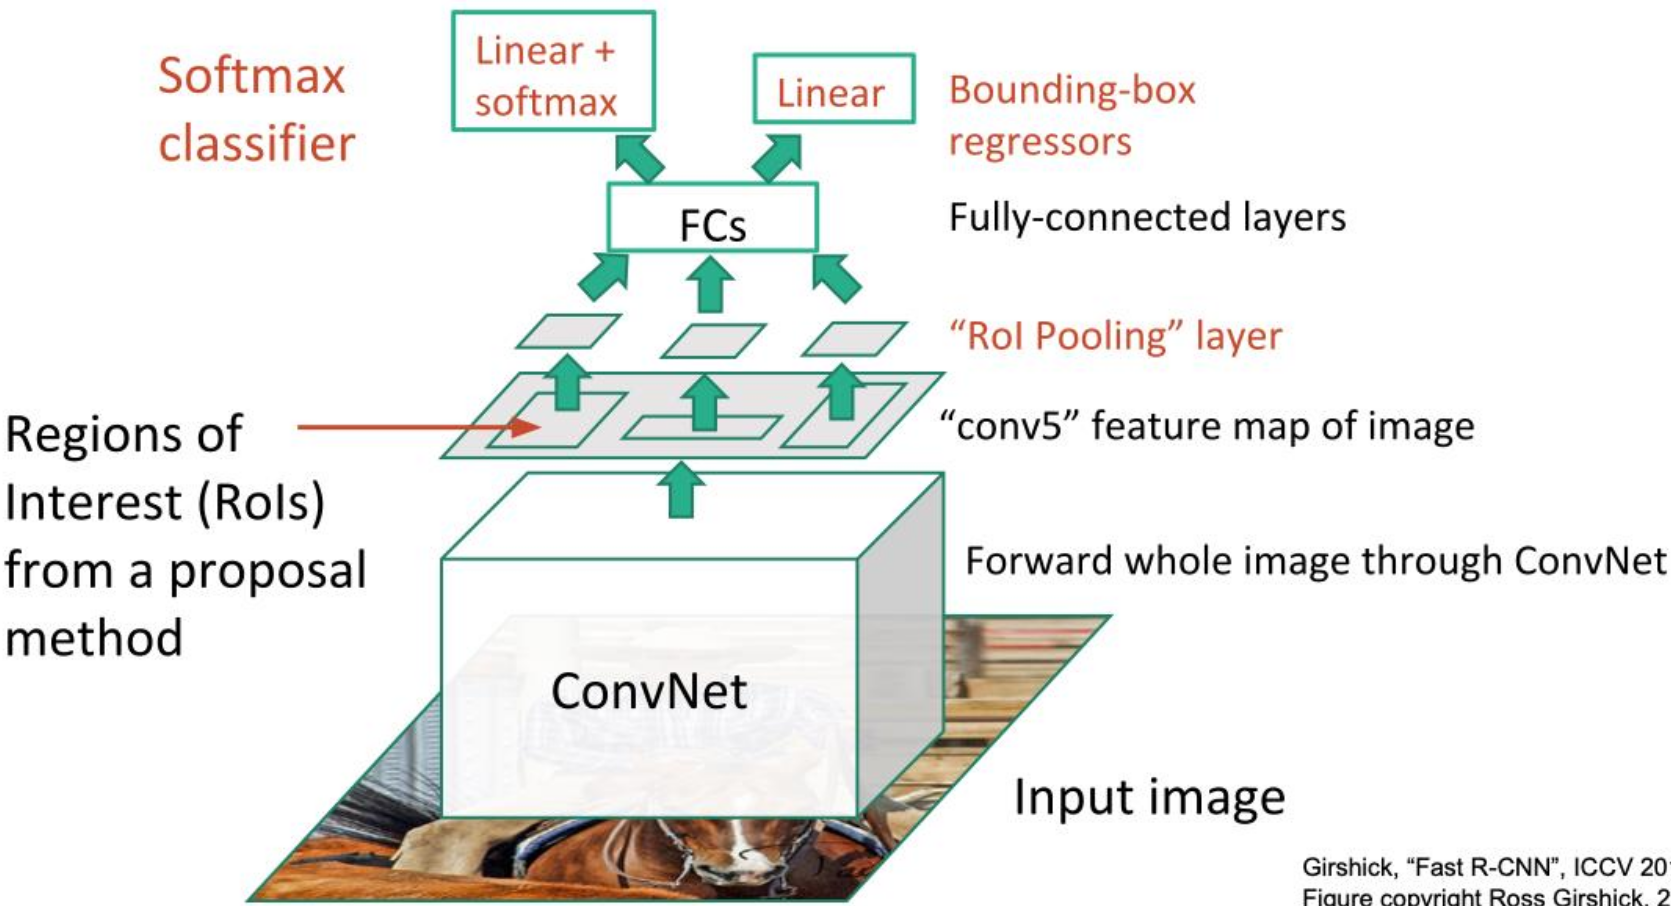
\includegraphics[width=1\textwidth]{sections/FindingMultipleObjects/img/fast_rcnn.png}
\end{minipage}
\begin{minipage}{0.5\textwidth}
    \paragraph{Faster RCNN}
    Replace proposal region function with fully convolutional network $\rightarrow$ Region Proposal Network (RPN)

    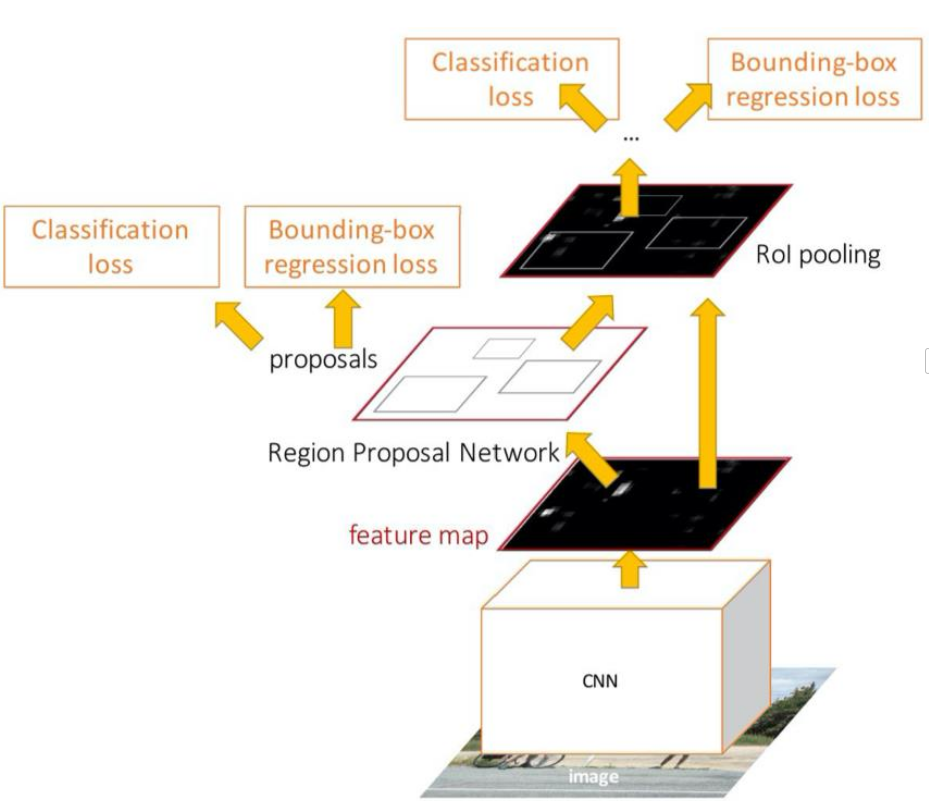
\includegraphics[width=0.7\textwidth]{sections/FindingMultipleObjects/img/faster_rcnn.png}
\end{minipage}

\subsubsection{Region-based Fully Convolutional Networks (R-FCN)}
\begin{itemize}
    \item 2 Stage strategy
          \begin{itemize}
              \item Region proposals by fully convolutional region proposal network (RPN) yields region of interests (ROI)
              \item Classification of ROIs into objects and background by fully convolutional network
          \end{itemize}
    \item ResNet 101 as base network (pretrained)
    \item Each ROI is divided into a grid, each grid cell gets a score
\end{itemize}

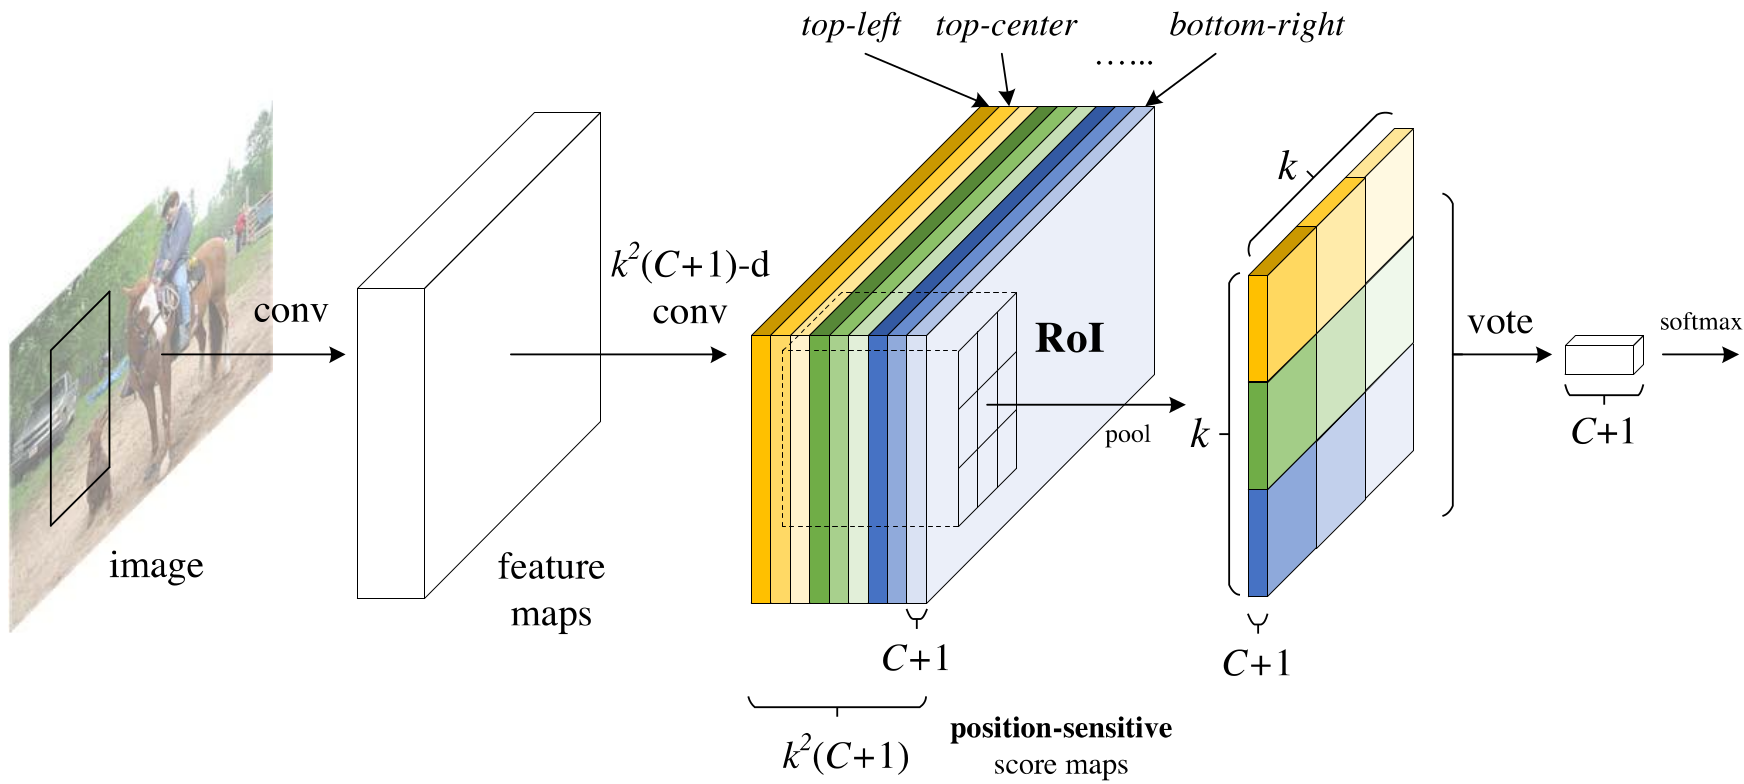
\includegraphics[width=.7\textwidth]{sections/FindingMultipleObjects/img/rfcn}


\subsubsection{You Only Look Once (YOLO)}
\begin{minipage}{0.5\textwidth}
    \begin{enumerate}
        \item Divide Image into $S\times S$ grid
        \item Each grid cell predicts $B$ bounding boxes with confidence scores ($x$, $z$, $w$, $h$, score)
        \item Each grid cell predics class probabilities (independent of bounding boxes)
        \item Multiply confidence score and probabilites at test time
    \end{enumerate}
    New version
    \begin{itemize}
        \item Add Batch Normalization
        \item Higher resolution ($448\times 448$)
        \item Use anchor bounding boxes from $k$-means analysis on the training data
        \item Use new base net (darknet 19 and darknet 58)
    \end{itemize}
\end{minipage}
\begin{minipage}{0.5\textwidth}
    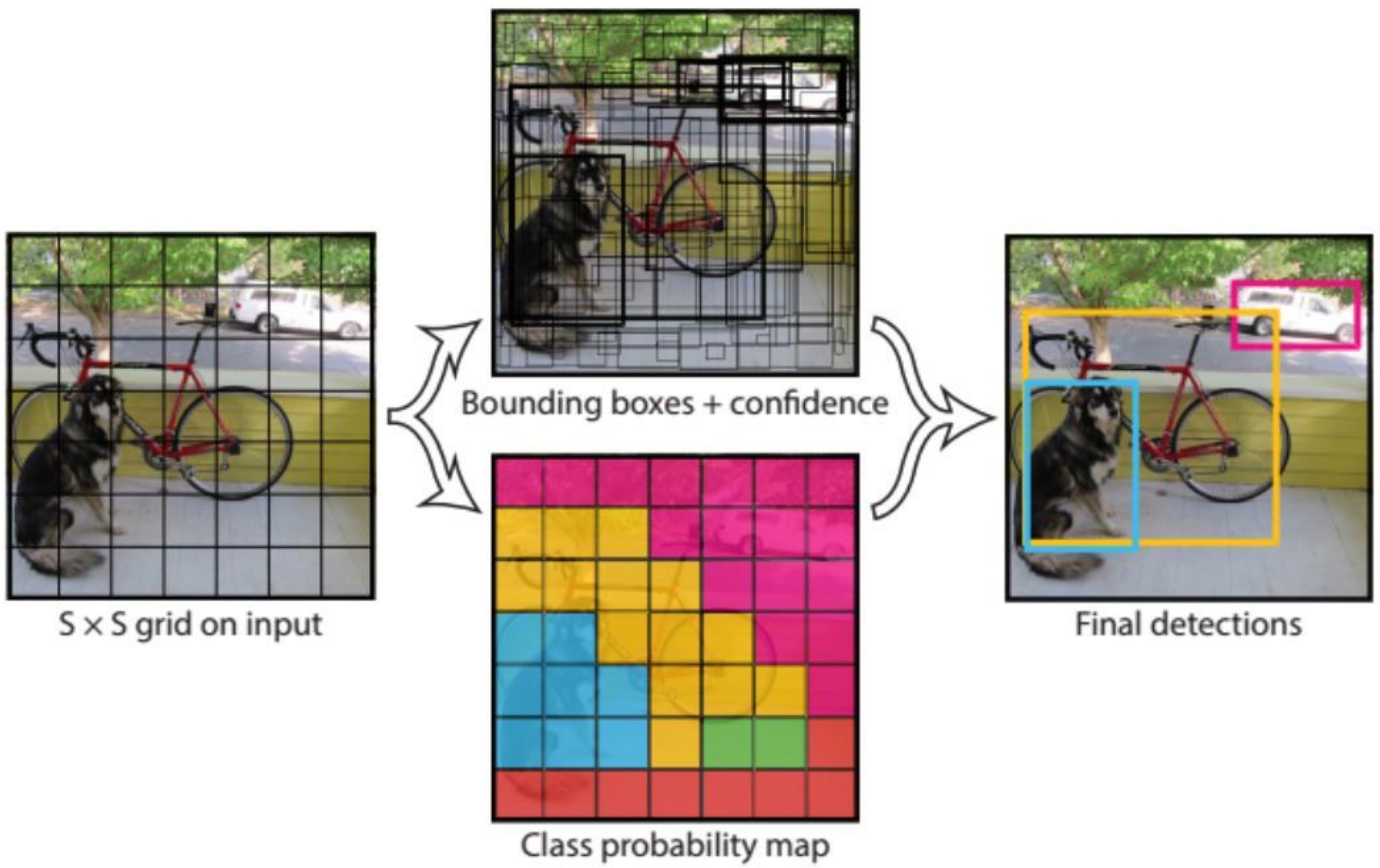
\includegraphics[width=1\textwidth]{sections/FindingMultipleObjects/img/yolo.png}
\end{minipage}
\clearpage
\textbf{Darknets 19 and 58}

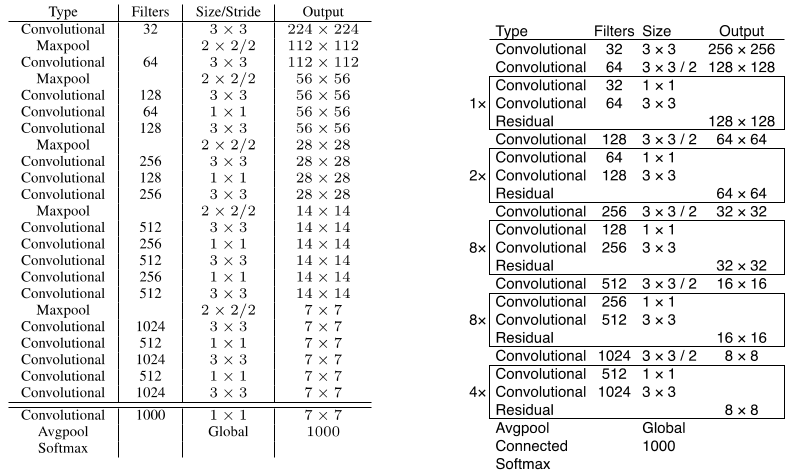
\includegraphics[width=.9\textwidth]{sections/FindingMultipleObjects/img/darknets.png}

\subsubsection{Single-Shot Detector (SSD)}
\begin{minipage}{0.5\textwidth}
    \begin{enumerate}
        \item Divide Image into $S\times S$ grid
        \item Use few standard bounding boxes for each grid cell
        \item Predict shape offset and confidence for each object class
        \item Faster and more accurate then YOLO (claim by the authors)
    \end{enumerate}
\end{minipage}
\begin{minipage}{0.5\textwidth}
    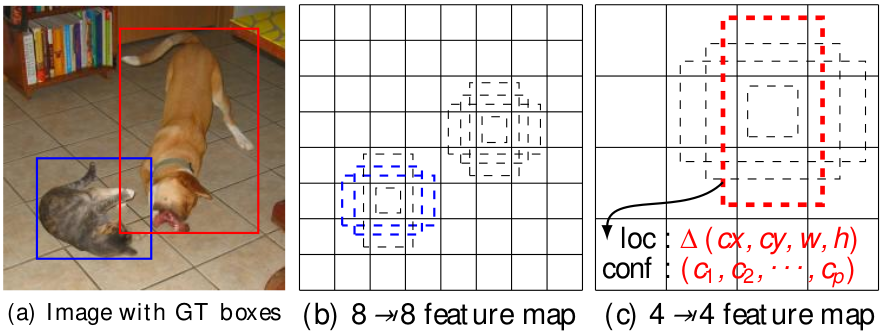
\includegraphics[width=1\textwidth]{sections/FindingMultipleObjects/img/ssd.png}
\end{minipage}

\subsubsection{CenterNet}
\begin{minipage}{0.5\textwidth}
    \begin{itemize}
        \item Model object as a single point (center of bounding box)
        \item Use key point estimation to find center point
        \item Use regression to find other properties (bounding box, orientation, etc.)
        \item Use network for keypoint preditction (at lower resolution)
        \item Use heatmap around ground true keypoint and use logistic regression as loss
        \item Use different backbone networke like ResNet (with additional upsampling) or hourglass
        \item Same base network to detect keypoint class and position (low resolution), offset and bounding box sizes.
        \item $f: [0,255]^{W \times H \times 3} \in \mathbb{N} \mapsto [0,1]^{W/R \times H/R \times C} \in \mathbb{R}$
    \end{itemize}
\end{minipage}
\begin{minipage}{0.5\textwidth}
    \centering
    Hourglass Network

    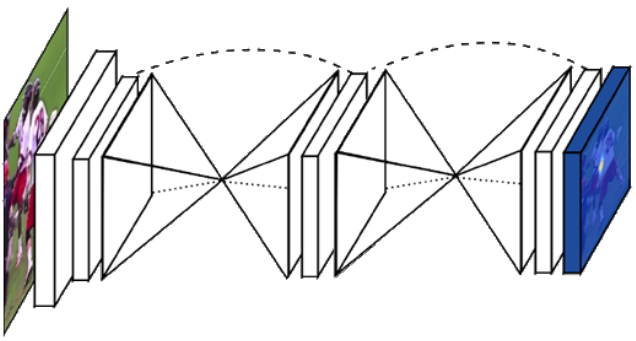
\includegraphics[width=\textwidth]{sections/FindingMultipleObjects/img/hourglass.png}
\end{minipage}
